\documentclass{deliverablereport}

\deliverable{component-architecture}{hpc-configure}
\deliverydate{XX/YY/201Z}
\duedate{31/08/2019 (M48)}
\author{Author names}

\begin{document}
\maketitle
% This will be the abstract, fetched from the github description
\githubissuedescription

% write the report here


%%%%%%%%%%%%%%%%%%%%%%%%%%%%%%%%%%%%%%%%%%%%%%%%%%%%%%%%%%%%%%
\section{Introduction}

%%%%%%%%%%%%%%%%%%%%%%%%%%%%%%%%%%%%%%%%%%%%%%%%%%%%%%%%%%%%%%
\section{Number Theory}

PARI-MT and the difficulty of composing a threaded systems into another.

%%%%%%%%%%%%%%%%%%%%%%%%%%%%%%%%%%%%%%%%%%%%%%%%%%%%%%%%%%%%%%
\section{Finite field linear algebra}
FFLAS-FFPACK

\begin{figure}
  \begin{center}
    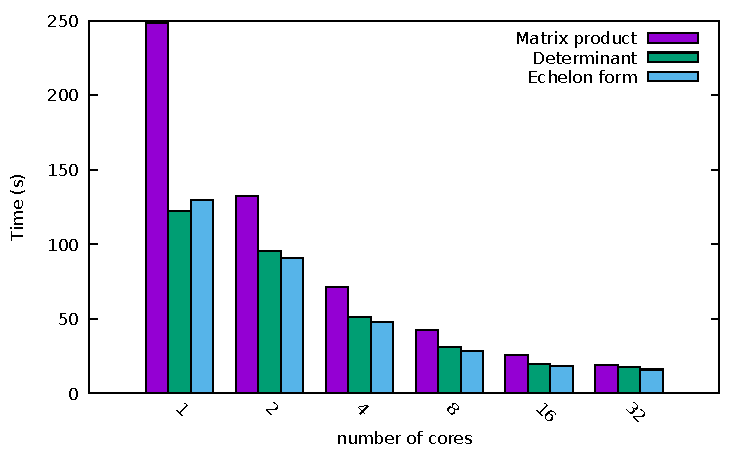
\includegraphics[width=.6\textwidth]{Pictures/histo_bigfoot3}
    \caption{Parallel speedup for some finite field linear algebra operations in SageMath}
  \end{center}
\end{figure}

\end{document}

%%% Local Variables:
%%% mode: latex
%%% TeX-master: t
%%% End:

